\documentclass
[
  12pt,
  handout,
  notes=show,
  svgnames		% für xcolor, datapie
]{beamer}

\usepackage[utf8x]{inputenc}
\usepackage{ucs}
\usepackage{amsmath}
\usepackage{amsfonts}
\usepackage{amssymb}
\usepackage{multicol}
\usepackage{graphicx}
%\usepackage{hyperref}		% automatic included by beamer
\usepackage{tikz}
\usetikzlibrary{arrows,positioning,shapes}
\usepackage{listings}
\usepackage{multicol}
\usepackage[absolute,overlay]{textpos}
\usepackage{appendixnumberbeamer}
\usepackage{url}

\setlength{\TPHorizModule}{1cm}
\setlength{\TPVertModule}{1cm}

\title{Embedded GNU/Linux Basics}
%\subtitle{}
\author{Urs Fässler}
\date{21.11.2015}
\institute
{
  17. LinuxDay\\
  Dornbirn
}
%\subject{}

\newcommand{\hnote}[1]{\only<handout>{\footnote{#1}}}
\newcommand{\hcite}[1]{\only<handout>{\cite{#1}}}
\bibliographystyle{plainurl}  % urlbst
\setbeamertemplate{bibliography item}{[\theenumiv]}

\lstset
{  
	basicstyle=\footnotesize\ttfamily,
	keywordstyle={\bf\color{green!50!black}},
	identifierstyle=\color{blue!25!black},
	stringstyle=\color{orange!75!black},
%  language=,
%  morekeywords={signals,slots,interface,event,message,String,Integer,component,import,uses,provides,implementation,connection,elementary,begin,end,func,pure,const},
%  numbers=none,
  numberstyle={\color{Grey}},
%  keywordstyle={\color{DarkRed}\bfseries},
%  identifierstyle={\color{Blue}}
%  columns=flexible,
  float=tb,
	frame=none,
}


\newcommand*\oldmacro{}%
\let\oldmacro\insertshorttitle%
\renewcommand*\insertshorttitle{%
	\oldmacro\hfill%
	\insertframenumber
}
\usetheme{Luebeck}

% remove navigation bars
\beamertemplatenavigationsymbolsempty

% remove section information
\setbeamertemplate{headline}{}

\begin{document}

\frame{\titlepage}

\begin{frame}{Wichtig}
	\begin{itemize}
		\item Involvierte Software (Firmware, u-boot, Linux, Treiber, Service-Management, Services)
		\item Boot-Prozess
		\item Workflow mit Yocto
	\end{itemize}
\end{frame}

\begin{frame}{Eigenschaften Embedded System\hcite{embeddedSpecials}}
	\pause
	\begin{multicols}{2}
		\begin{itemize}
			\item Kosten
			\item Grösse
			\item Energie
			\item Zuverlässigkeit
			\item Sicherheit
			\item Langlebigkeit
			\item Echtzeit
		\end{itemize}
	\end{multicols}
\end{frame}

\begin{frame}{Definition Embedded System}
	Der Ausdruck embedded system bezeichnet einen Computer, der in einem technischen Kontext eingebettet ist. \hcite{wikiEmbedded}
	\begin{flushright}
		Nach Wikipedia
	\end{flushright}
\end{frame}

\begin{frame}{Embedded Systeme}
	\footnotesize{
	\begin{multicols}{2}
				\only<handout>{Digitales Multimeter}
				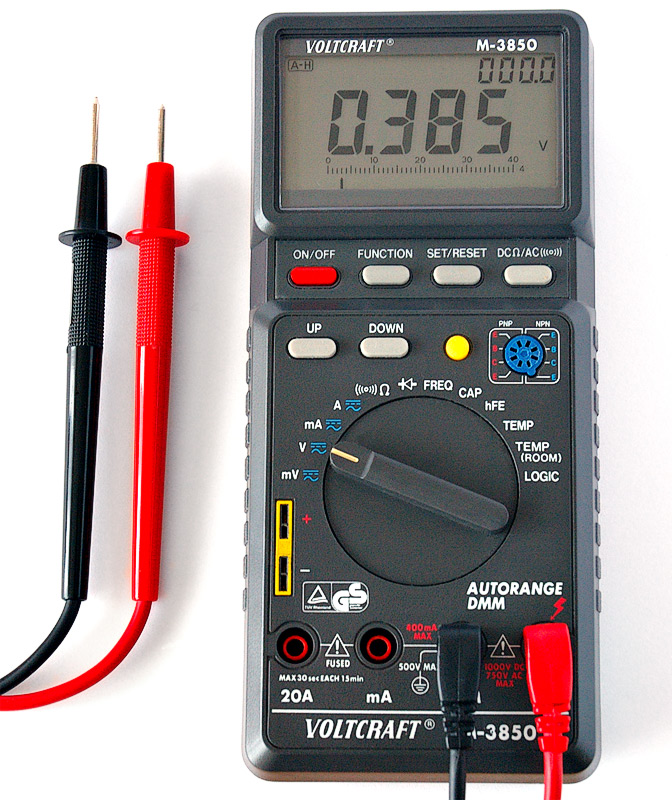
\includegraphics[height=4cm]{res/Digital_Multimeter_Aka.jpg}\hcite{multimeter}
				\only<handout>{
					\begin{itemize}
						\item Sensor produziert ~20 B/sec
						\item Reduzierung auf ~2 B/sec
						\item Verarbeitung auf internem uC
					\end{itemize}
				}
				\pagebreak
				\only<handout>{ATLAS/LHC/CERN}
				\visible<2->{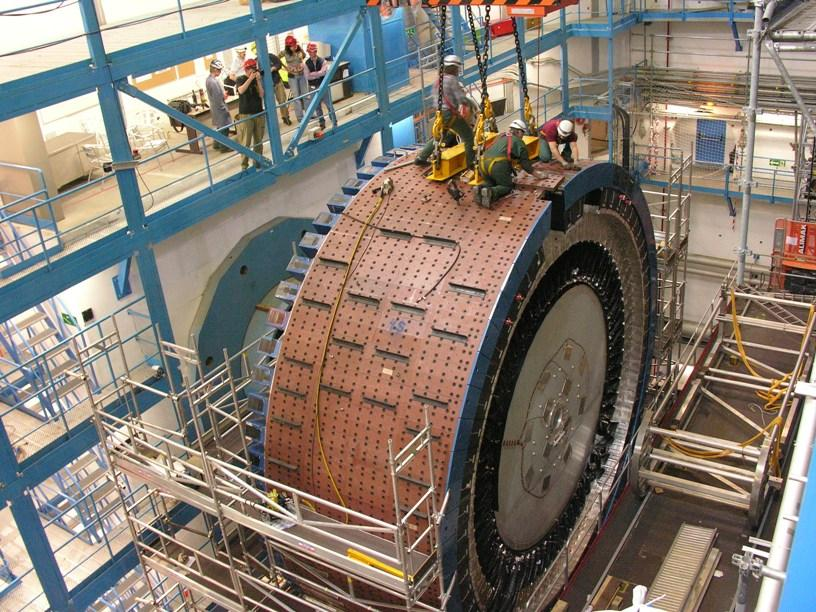
\includegraphics[height=4cm]{res/ATLAS_Tile_Calorimeter}\hcite{tileCalorimeter}}
				\only<handout>{
					\begin{itemize}
						\item Sensor produziert 1 PiB/sec
						\item Reduzierung auf ~100 MiB/sec \hcite{wikiAtlas}
						\item Verarbeitung auf eigenen 20'000 Server und Grid \hcite{wikiCernServer}
					\end{itemize}
				}
	\end{multicols}
	}
\end{frame}

\begin{frame}{Typisches GNU/Linux Embedded System}
	\begin{center}
		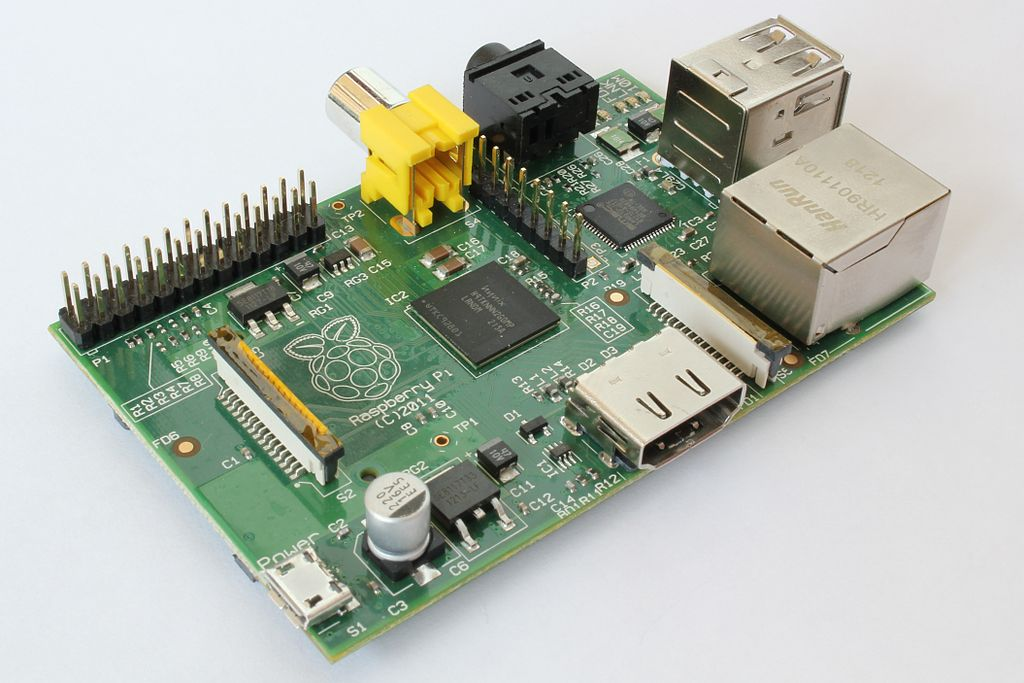
\includegraphics[width=5cm]{res/RaspberryPi.jpg}\hcite{raspberryPi}
		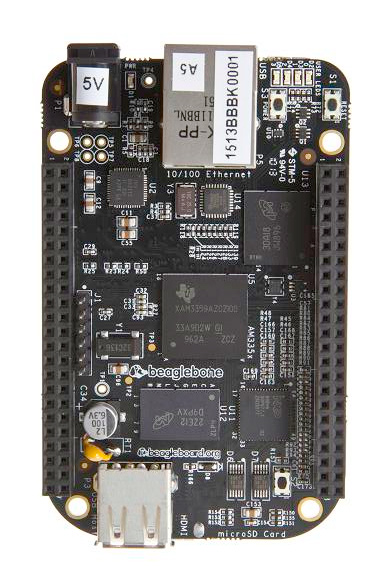
\includegraphics[width=3.5cm]{res/Beaglebone_Black.jpg}\hcite{beagleboneBlack}
	\end{center}
\end{frame}

\begin{frame}{Echtzeit}
	\begin{center}
		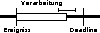
\includegraphics[width=8cm]{res/echtzeit.pdf}
	\end{center}
	\only<handout>{
		\begin{itemize}
			\item Bearbeitung ist nach einer bestimmten Zeit nach dem auftreten eines Ereignisses abgeschlossen.
			\item bei weicher Echtzeit ist dieses Verhalten wünschenswert (Video Wiedergabe)
			\item Echtzeit ist oft nicht nötig
			\item Linux ist nicht Echtzeit-Fähig
			\item Lösung ist separater uC, im SOC oder dediziertem Chip
		\end{itemize}
	}
\end{frame}



\begin{frame}{Boot Process \cite{OMAPBootloaderOverview}}
	\begin{tabular}{|l|l|l|}
		\hline typ & name & funktion \\ 
		\hline system startup & ROM Code & minimal hardware initialisierung \\ 
		& & in boot devices nach image suchen \\
		& & stage 1 loader ins ram laden und ausführen \\
		
		\hline stage 1 loader & x-loader (u-boot) & pin muxing \\ 
		& & clock und memory initialisieren \\
		& & stage 2 loader ins ram laden und ausführen \\
		
		\hline stage 2 loader & u-boot & platform initialisierung (USB, Netzwerk, \ldots) \\
		& & boot menu / Kommandozeile anzeigen \\
		& & Kernel und Device-Tree ins ram laden und ausführen \\
		
		\hline kernel & Linux & Treiber für Hardware laden \\ 
		& & root file system mounten \\
		& & init process starten \\
		
		\hline init & Systemd & Abhängigkeiten zwischen Services auflösen \\ 
		& & Services starten \\
		& & Services überwachen \\
		
		\hline 
	\end{tabular} 
\end{frame}


\begin{frame}{Wann/Wieso Linux}
	Gegenueber einem uC wie Arduino bringt GNU/Linux
	\begin{itemize}
		\item Hardware-Treiber
		\item Protokolle
		\item Tools
		\item erhoehte Komplexitaet
	\end{itemize}
\end{frame}

\begin{frame}{Hardware auswahl}
	\begin{itemize}
		\item Eval-/Bastelboards (Raspi, BeagleBone)
		\item Consumer Hardware (Router, Media-Center, \ldots)
		\item Profesionelle Boards
	\end{itemize}
\end{frame}

\begin{frame}{Echtzeit}
	\begin{itemize}
		\item Bearbeitung ist nach einer bestimmten Zeit nach dem auftreten eines Ereignisses abgeschlossen.
		\item Die Bearbeitung eines Interrupts dauert nie laenger als $t$.
		\item bei weicher Echtzeit ist dieses Verhalten wuenschenswert (Video wiedergabe)
		\item jeder Treiber kann Interrupts sperren
		\item Swapping
		\item Prozessoren mit Caches haben undefinierbares Verhalten, abschalten nicht Sinn der Sache
		\item Loesung ist separater uC, im selben oder eigenen DIE
	\end{itemize}
\end{frame}

\begin{frame}{Firmware}
	``Unter Firmware versteht man Software, die in elektronische Geräte eingebettet ist.'' \cite{wikiFirmware}
	
	\begin{itemize}
		\item Geamtes Software-Image von Embedded System
		\item Software fuer subsyteme
		\begin{itemize}
			\item Power Management
			\item WLAN Karte
			\item BIOS
			\item Touch-Screen
		\end{itemize}
	\end{itemize}
	
	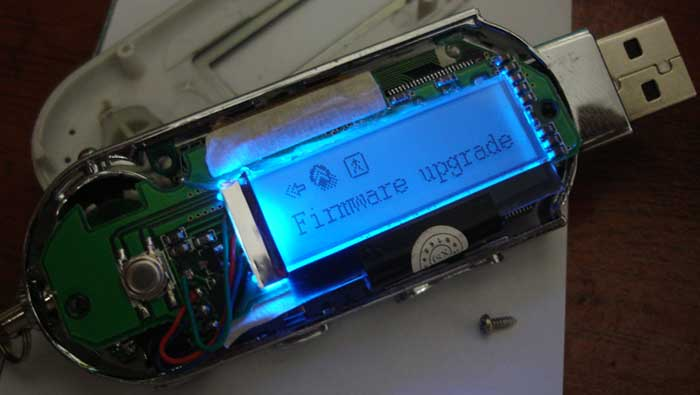
\includegraphics[height=2cm]{res/Firmware_upgrade.jpg} \cite{firmwareUpgrade}
\end{frame}

\begin{frame}{PID 1}
	Nachdem Linux alles initializiert hat wird Kontrolle an Userspace uebergeben.
	Ueblicherweise ist dies systemd.
	\begin{itemize}
		\item systemd
		\begin{itemize}
			\item einfach da bekannt
			\item wenn mehrere Dienste noetig
			\item gewisse groesse
		\end{itemize}
		\item script
		\begin{itemize}
			\item wenn nur wenige Dienste
		\end{itemize}
		\item applikation
		\begin{itemize}
			\item Applikation muss alles machen
			\item nur fuer monolithische Applikationen
		\end{itemize}
	\end{itemize}
\end{frame}

\begin{frame}{Yocto}
	Aufgaben um Embedded system zu erstellen
	\begin{itemize}
		\item Cross Compiler bauen
		\item sysfs bauen (Kernel und benoetigte Tools fuer system)
		\item Cross Compiler und sysfs fuer Developer bereitstellen (sdk)
	\end{itemize}
	Aufgaben um Embedded system zu deployen
	\begin{itemize}
		\item Applikation cross-compilen
		\item sysfs cross-compilen
		\item Kernel cross-compilen
		\item applikationen packetieren
		\item image zusammenstellen
	\end{itemize}
	daher Yocto (Yocto Workflow zeigen, resp. bild aus fsfe präsentation)
\end{frame}

\begin{frame}{Kernel / Linux}
	\begin{itemize}
		\item Verteilen von Resourcen
		\item Initialisieren und Abstrahieren der Hardware
	\end{itemize}
\end{frame}

\begin{frame}{Device Tree}
	\begin{itemize}
		\item meiste Hardware ist nicht Plug and Play
		\item wir muessen Linux mitteilen, wo welche Hardware liegt
		\item Device Tree listet auf, wo sich welche Hardware befindet
		\item Linux laedt Treiber anhand Infos in Device Tree
	\end{itemize}
	\begin{itemize}
		\item Struktur aehnlich wie XML
		\item gegliedert nach BUS
		\item beschreibt welche Hardwrae angeschlossen ist
		\item Hierarchisch aufgebaut wie Hardware (SOC, Modul, Geraet, System)
	\end{itemize}
	Beispiel
\end{frame}



\section{Beispiel}

\begin{frame}{Aufgabe}
	\begin{itemize}
		\item Webserver für Most Useless Machine Ever!
	\end{itemize}
	\begin{center}
		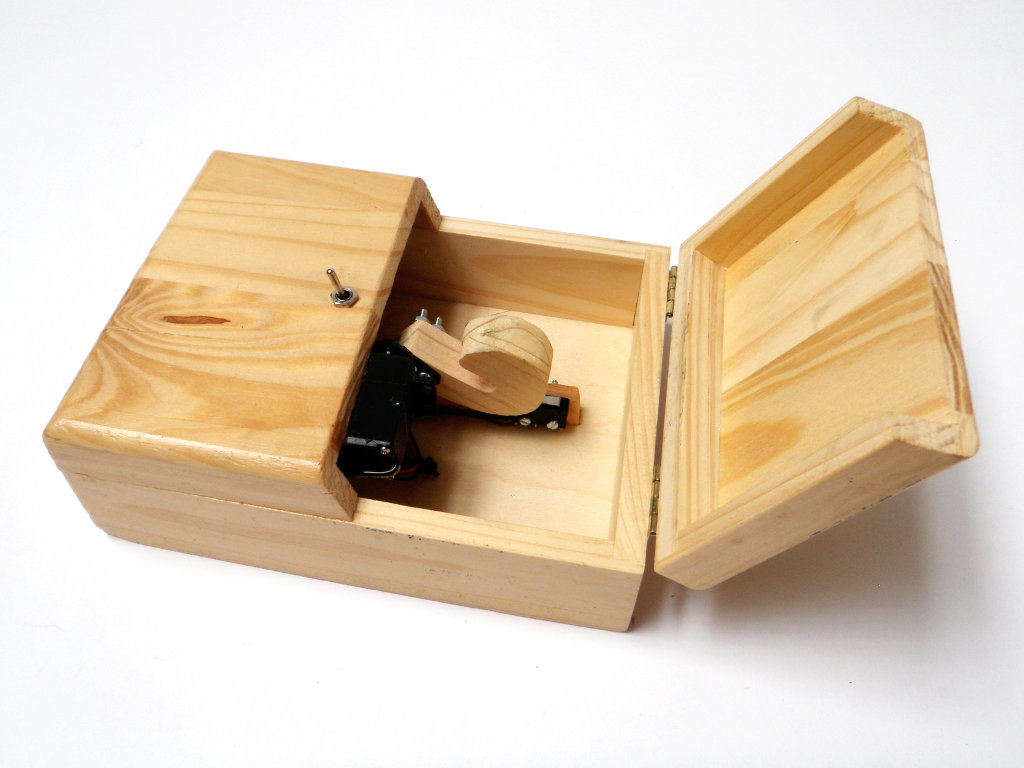
\includegraphics[width=0.75\textwidth]{res/mume.jpg}
		\cite{mumePic}
	\end{center}
\end{frame}

\begin{frame}{System}
	\begin{itemize}
		\item uC oder GNU/Linux?
		\item Gegenüber einem uC wie Arduino bringt GNU/Linux
		\begin{itemize}
			\item Hardware-Treiber
			\item Protokolle
			\item Tools
			\item erhöhte Komplexität
		\end{itemize}
	\end{itemize}
\end{frame}

\begin{frame}{Hardware}
	\begin{itemize}
		\item Eval-/Bastelboards (Raspi, BeagleBone)
		\item Consumer Hardware (Router, Media-Center, \ldots)
		\item Profesionelle Boards
		\item[$\rightarrow$] BeagleBone Green
		\begin{itemize}
			\item Netzwerk
			\item USB
			\item Yocto Supported
			\item viele Anshlüsse
			\item USB Powered
			\item kein Display Anschluss
			\item bereits Erfahrung
		\end{itemize}
	\end{itemize}
\end{frame}

\begin{frame}{Developer Image}
	\begin{itemize}
		\item Wie kriegen wir ein Linux drauf?
		\item[$\rightarrow$] Yocto
	\end{itemize}
\end{frame}

\begin{frame}{SDK}
	\begin{itemize}
		\item Wie können wir Software dafür kompilieren?
		\item[$\rightarrow$] Yocto SDK
		\begin{itemize}
			\item cross compiler
			\item root file system
		\end{itemize}
	\end{itemize}
\end{frame}

\begin{frame}{Treiber}
	\begin{itemize}
		\item wie können wir die Hardware ansteuern?
		\item[$\rightarrow$] Linux Treiber
		\begin{itemize}
			\item GPIO
			\item PWM
			\item sysfs
			\item Device-Tree
		\end{itemize}
	\end{itemize}
\end{frame}

\begin{frame}{MUME Service}
	\begin{itemize}
		\item wie können wir mit dem Treiber kommunizieren?
		\item[$\rightarrow$] sysfs / D-Bus
		\begin{itemize}
			\item Service der den Treiber weiter abstrahiert
		\end{itemize}
	\end{itemize}
\end{frame}

\begin{frame}{GUI}
	\begin{itemize}
		\item Koennen wir via Browser auf das System zugreifen?
		\item[$\rightarrow$] gui
		\begin{itemize}
			\item nginx
			\item fastcgi
			\item gui
			\item D-Bus
		\end{itemize}
	\end{itemize}
\end{frame}

\begin{frame}{Service Manager}
	\begin{itemize}
		\item Wie starten und managen wir die Services?
		\item[$\rightarrow$] systemd
		\begin{itemize}
			\item service files schreiben
			\item fastcgi
			\item gui
			\item D-Bus
		\end{itemize}
	\end{itemize}
\end{frame}

\begin{frame}{Produktiv Image}
	\begin{itemize}
		\item Wie können wir die Firmware verteilen?
		\item[$\rightarrow$] Yocto
	\end{itemize}
\end{frame}







\begin{frame}{system}
	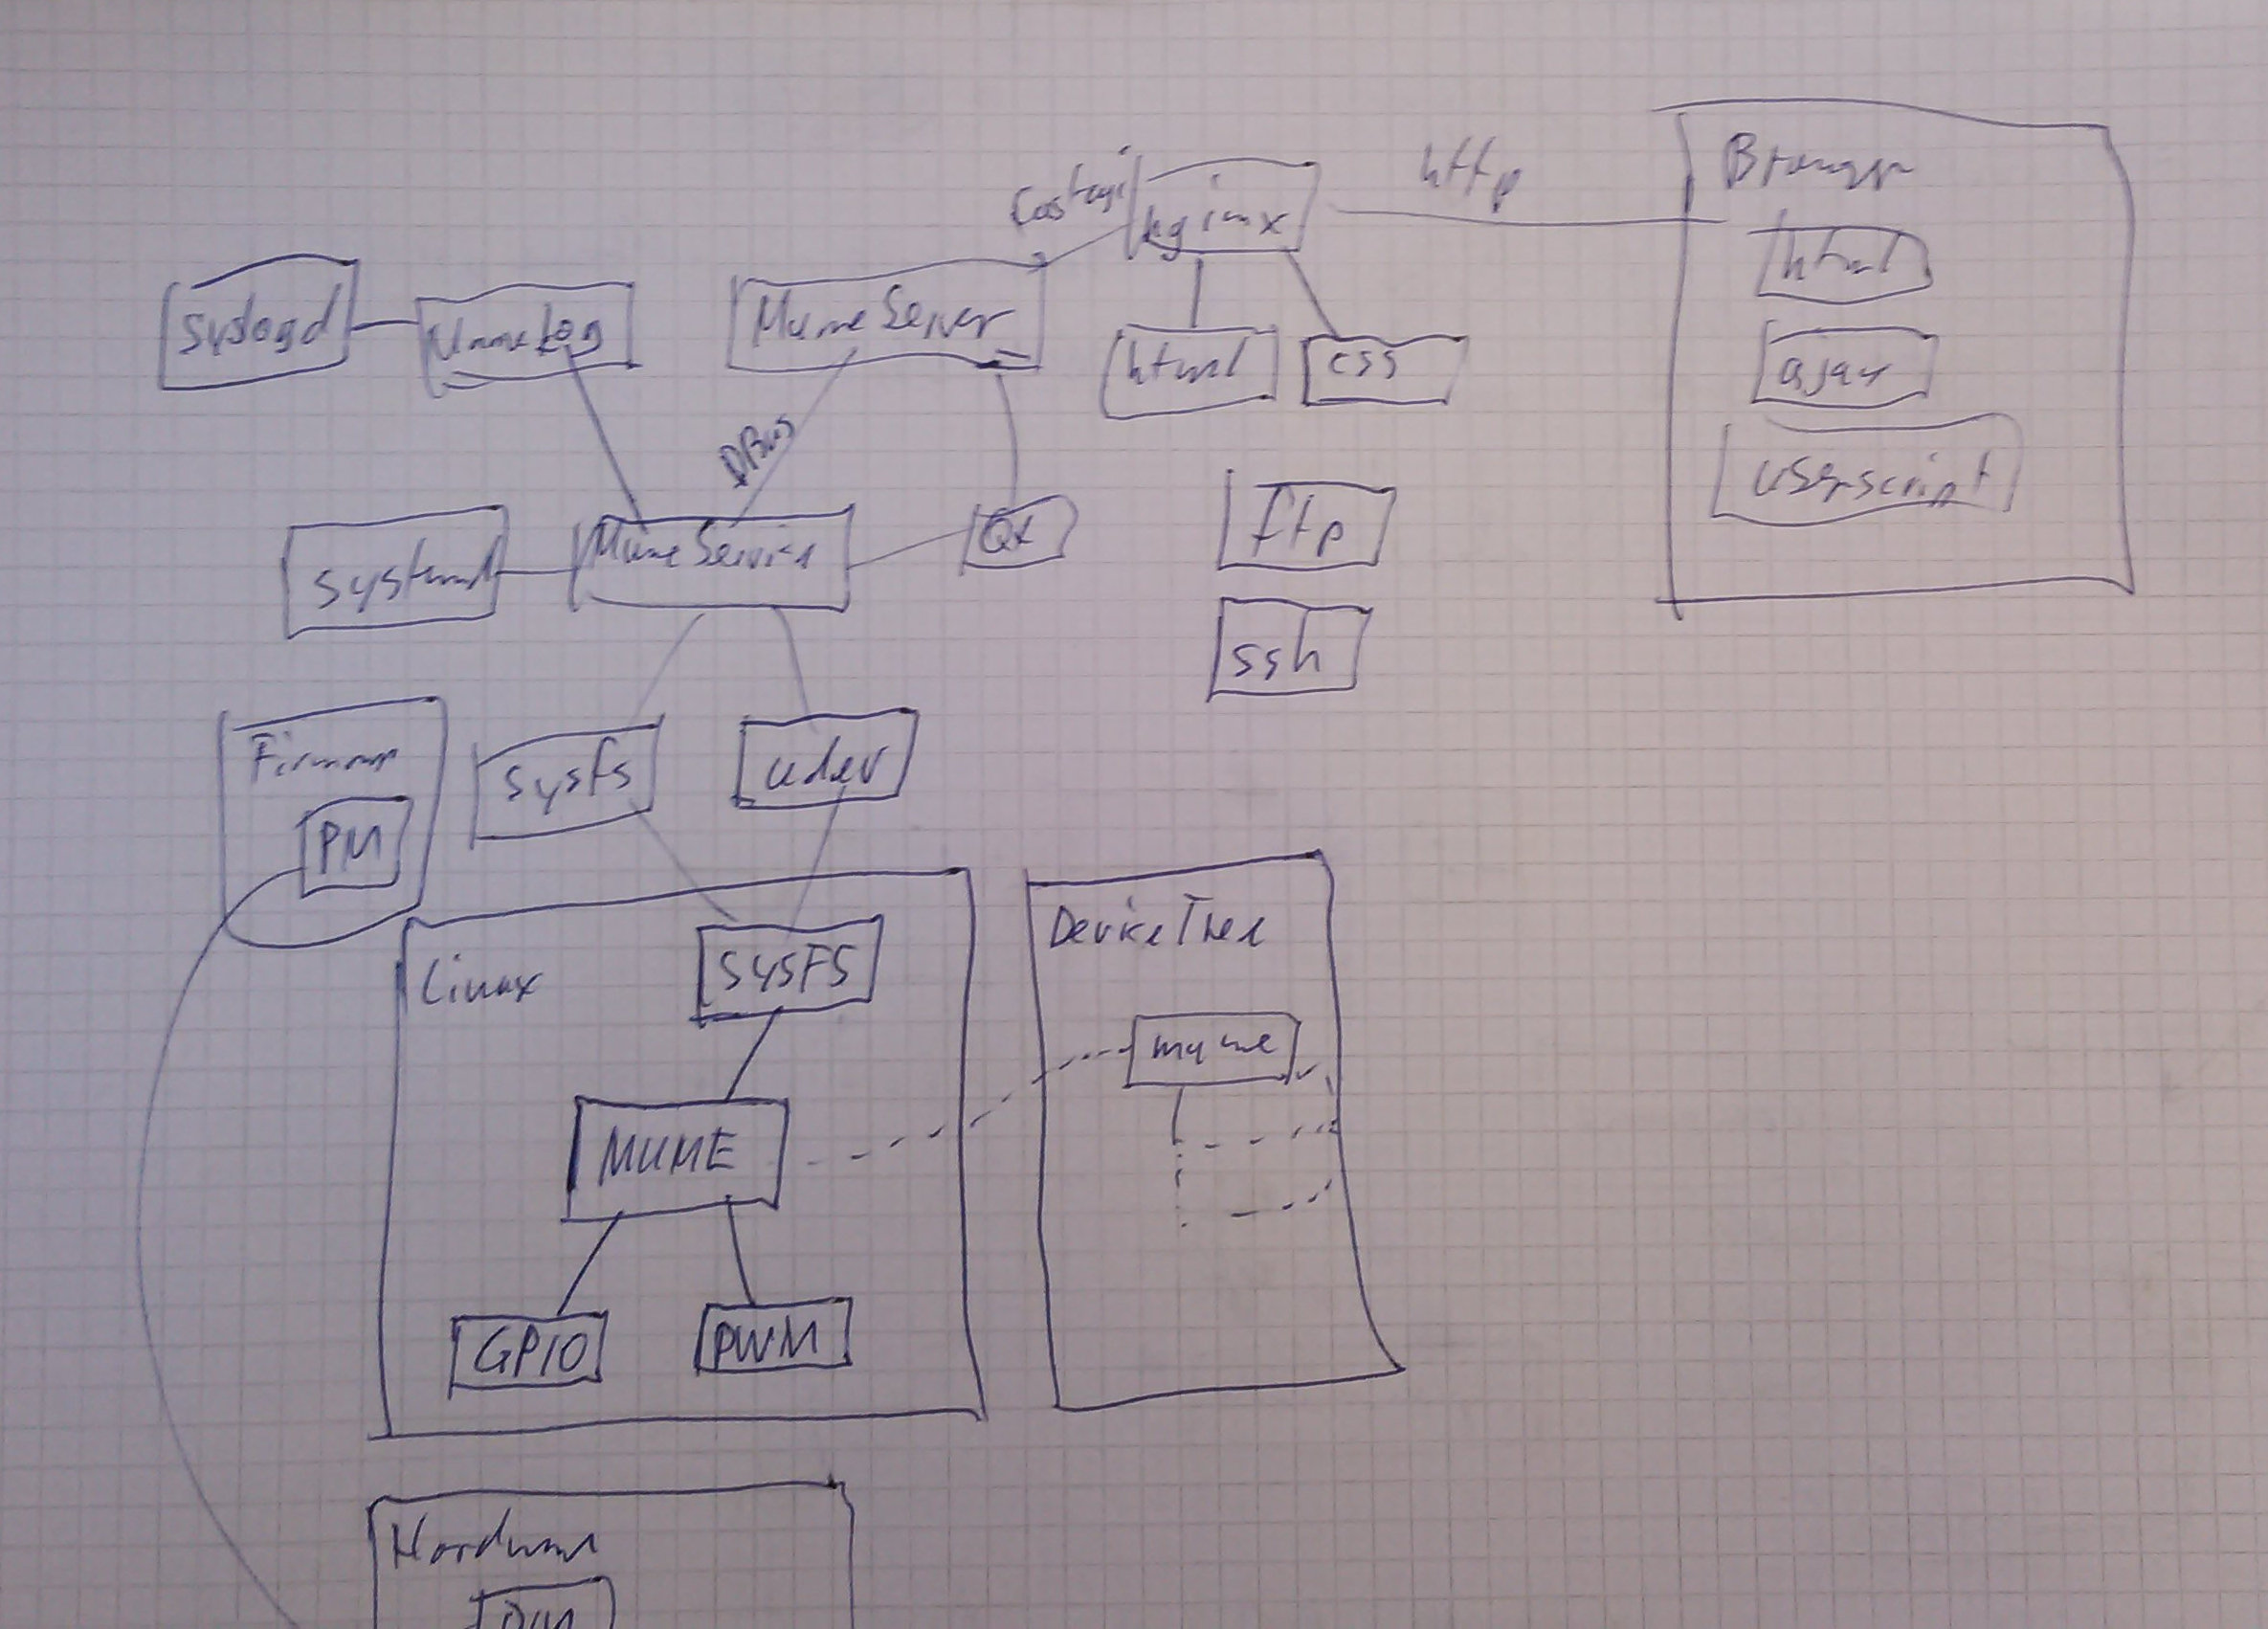
\includegraphics[width=\textwidth]{res/system.jpg}
\end{frame}

\begin{frame}{Linux}
	\begin{itemize}
		\item Sammlung von Subsystemen, abstraktionenen
		\item i2c
		\item spi
		\item iio
		\item fbtft
		\item gpio
		\item led
	\end{itemize}
\end{frame}

\begin{frame}{eigener Treiber}
	Beispiel ``Most Usless Machine Ever''
\end{frame}

\begin{frame}{Applikationen}
	Siehe System
	\begin{itemize}
		\item Embedded System besteht meist aus mehreren Prozessen $\rightarrow$ Microservices
		\item Webserver, Prozessueberwachung, SSH, FTP, UI
		\item gutes IPC system (z.B. kdbus)
		\item eigener Service
		\begin{itemize}
			\item reaktiv, event-getriggert
			\item Qt gut geeignet
			\item andere Frameworks moeglich
			\item auch ohne Framework moeglich
		\end{itemize}
	\end{itemize}
\end{frame}

\begin{frame}{Webserver}
\end{frame}


\begin{frame}{Sonstiges}
	\begin{itemize}
		\item[busybox] Reimplementation von GNU/Linux Tools in einem Binary, optimiert auf groesse; oft eingeschraenker Funktionsumfang
	\end{itemize}
\end{frame}


\only<handout>
{
\appendix

\begin{frame}[allowframebreaks]{Literature}
	\bibliography{literature}
\end{frame}

}

\end{document}
